\documentclass{article} % For LaTeX2e
\usepackage{nips14submit_e,times}
\usepackage{hyperref}
\usepackage{url}
\usepackage{graphicx}
\usepackage{caption}
\usepackage{subcaption}

\newenvironment{itemizedense}{
\begin{itemize}
  \setlength{\itemsep}{1pt}
  \setlength{\parskip}{0pt}
  \setlength{\parsep}{0pt}
}{\end{itemize}}

%\documentstyle[nips14submit_09,times,art10]{article} % For LaTeX 2.09

\title{DS-GA-1008 Assignment 2: Team LongCat}

\author{
Catherine Olsson, Long Sha, and Kevin Brown \\
}

\newcommand{\fix}{\marginpar{FIX}}
\newcommand{\new}{\marginpar{NEW}}

\nipsfinalcopy % Uncomment for camera-ready version

\begin{document}

\maketitle

\begin{abstract}
Overall, we implemented two main strategies: one basic supervised-learning
strategy, and one unsupervised-feature-learning strategy based on Dosovitskiy
et al. TODO REFERENCE. TODO what performance was achieved with each?
\end{abstract}

\section{Supervised-only network}

\subsection{Architecture}
TODO update this!

The input size is 3 color channels, and 96-by-96 pixels. 

TODO remaining layers

\subsection{Training}

TODO verify that the following is true!
We preprocessed the images by subtracting the global mean for each channel, and dividing by the standard deviation (zscore), for the train data. We then used this mean and standard deviation to transform the test data (to keep training and testing data separate).

No data augmentations were used. We used a dropout probability of 0.5 on the third layer. We used stochastic gradient descent with the following parameter values:

TODO check that the following are right

\begin{itemizedense}
\item Learning Rate $1 \times 10^{-7}$
\item Momentum of $0$
\item Weight decay of $0$
\item Loss function: negative log likelihood (nll)
\item TODO train/validation split
\end{itemizedense}

\subsection{Results}

TODO submit results!

\section{Unsupervised feature-learning network}

\subsection{Overview of approach}

The unsupervised feature-learning approach proceeds in two steps. The first step is to learn a feature representation from the unlabeled data. This is achieved by generating ``surrogate classes'', each consisting of a single image patch with various distortions applied, and then training a network to discriminate these surrogate classes. The second step is to train a classifier on the true labeled data, after first transforming the labeled images to the new feature representation.

\subsection{Step 1: Unsupervised feature learning}

\subsubsection{Surrogate data generation}

A surrogate dataset is generated by transforming patches of images drawn from the unlabeled image set. For each of the $n$ surrogate classes, a random image is chosen, a candidate 32x32 seed patch is selected, and $m$ exemplar patches are generated by applying random transformations to the original image.

First, candidate seed patches were screened for having enough variation in intensity, to avoid selecting uniform feature-less patches. We achieved this by filtering each candidate patch with a simple horizontal and vertical gradient filter (namely ${{1, 0, -1}}$ and ${{1},{0},{-1}}$). We set a minimum threshold for the overall sum of the absolute values of the pixel intensities in the two filtered images. Candidate patches which did not surpass this threshold were rejected. We found that a setting of $600$ produced interesting patches without taking too long to complete the search. 

Second, we generated $m$ transformed patches by randomly applying the following transformations:

\begin{itemizedense}
\item Rotation: up to 20 degrees, i.e. 0.35 radians.
\item Contrast: Raise the S and V components to a power between 0.25 and 3; multiply by 0.7 through 1.4; add -0.1 to 0.1.
\item Hue: add a value between -0.1 and 0.1
\item Translation: within 0.2 of the patch size
\end{itemizedense}

We did not implement the PCA-based contrast transformation described in Dostovitskiy et al, because it was more complicated to implement. We also removed the scaling transformation described in Dostovitskiy et al. simply because it was buggy and causing problems, and we did not have time to fix it before submission. We believe our results would have been more robust and our filters more scale-invariant if we had succeeded at implementing the scale transformation. We also added a left-right flip, which unfortunately was not quite correctly implemented; implementing this correctly may have gained us even better performance.

We experimented with using surrogate datasets with TODO RANGE N surrogate classes, each with TODO RANGE M exemplars. Consistent with the graphs in the original paper, we found that including more classes and more exemplars improved performance. However, the total number of classes and exemplars we were able to use was ultimately restricted by memory limitations in our current implementation. We settled on TODO N classes and TODO M exemplars for our final analysis.

\begin{figure}[h]
\centering
\begin{subfigure}{0.3\textwidth}
  \centering
  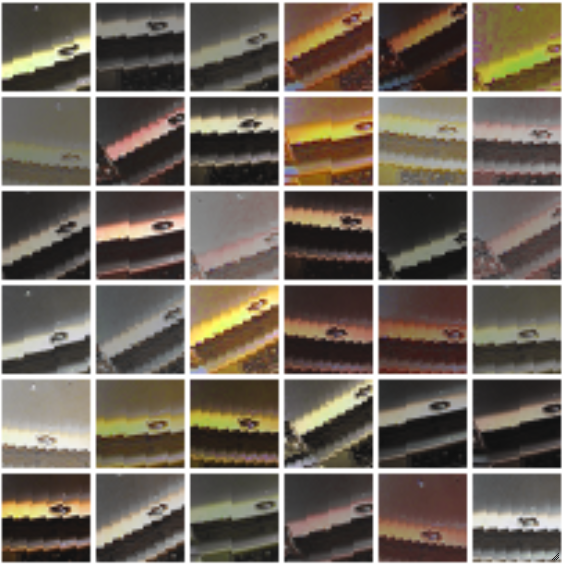
\includegraphics[width=\textwidth]{figs/patch_noflip_lines.png}
\end{subfigure}
\begin{subfigure}{0.3\textwidth}
  \centering
  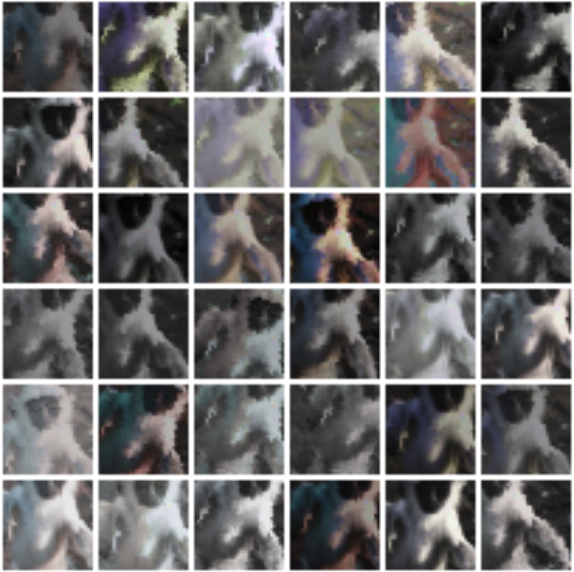
\includegraphics[width=\textwidth]{figs/patch_noflip_lemur.png}
\end{subfigure}
\begin{subfigure}{0.3\textwidth}
  \centering
  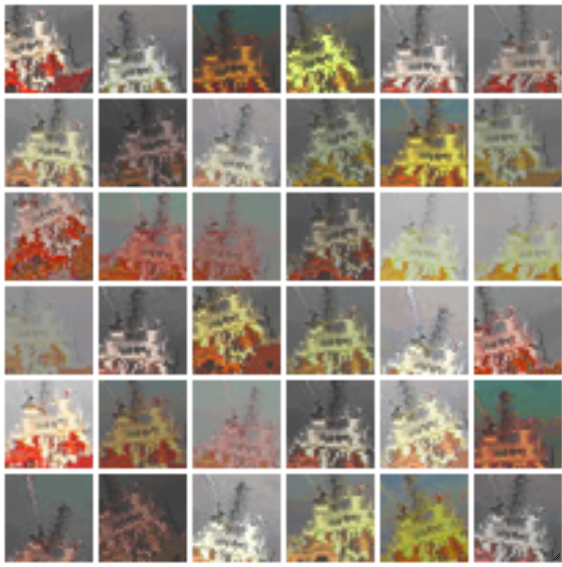
\includegraphics[width=\textwidth]{figs/patch_noflip_boattop.png}
\end{subfigure}
\label{figpatch}
\caption{A selection of exemplars from three surrogate classes}
\end{figure}

\subsubsection{Feature representation training}
The input of the feature representation training step is a surrogate dataset of $n$ generated classes, each with $m$ images (32x32) derived from each class' seed patch.

TODO what preprocessing?

The architecture of the surrogate-data classification model consists of three layers: (1) a 5x5 convolutional layer, stride of 1, with 128 filters, followed by a 2x2 max pool; (2) a second 5x5 convolutional layer, stride of 1, now with 256 filters, again followed by a 2x2 max pool; (3) a fully connected layer, with 512 outputs, using dropout of 0.5; finally, a linear mapping to the 10 output classes.

We used stochastic gradient descent, with the following parameter values:

\begin{itemizedense}
\item Learning Rate $1 \times 10^{-3}$
\item Momentum of $0$
\item Weight decay of $0$
\item Loss function: negative log likelihood (nll)
\item Training set is 75\% of the data; validation set is a random 25\%
\end{itemizedense}

We implemented the ability to perform ten-fold cross-validation, but did not use it for model selection because it proved to be very slow.

\subsection{Step 2: Supervised classification}

\subsubsection{Feature representation transformation}

As in Dosovitskiy et al., the next step after learning a network that can produce a feature representation is to train a \emph{second} network to discriminate the true labeled classes based on the new feature embedding.

In Dosovitskiy et al., they ``convolutionally compute the responses of all the network layers except the top softmax''. We interpreted this to mean that we should repeatedly run the learned model on 32x32 patches of each 96x96 image; and then concatenate the outputs of the first convolutional layer, the second convolutional layer, and the final fully connected layer to form a feature embedding of each patch. 

- Add spatial four-quadrant max pooling to the first layer and the second layer output to reduce dimensionality (e.g. from 128x14x14 to 128x2x2 after the first layer).
- Used a larger stride, to compute fewer patches in the image. We used a stride of 8, which reduced the number of patches per image from $65x65=4225$ patches to $9x9 = 81$ patches.
- Added a second spatial four-quadrant max pooling to the overall representation, reducing it from $(9*9) * (128 * 2 * 2 + 256 * 2 * 2 + 512)$ features to $(2*2) * (128 * 2 * 2 + 256 * 2 * 2 + 512)$
- Our final feature embedding per image was thus $8192$ dimensions.

\subsubsection{Supervised training}

Preprocessing TODO. Architecture TODO.

We used a dropout probability of 0.5 on the third layer. We used standard stochastic gradient descent, with the following parameter values:

\begin{itemizedense}
\item Learning Rate $1 \times 10^{-3}$
\item Momentum of $0$
\item Weight decay of $0$
\item Loss function: negative log likelihood (nll)
\item Training set is 75\% of the data; validation set is a random 25\%
\end{itemizedense}

\subsection{Results}

TODO fill in final results!

(Any conditions/variations we tried? How did they do?)

Adding the gradient cutoff in patch selection substantially improved our performance (from approximately 40\% to approximately 48\% on the validation set at the time we chose to include it).

We initially chose 128 filters per layer at all three layers. Our performance improved when we increased the dimensionality of the layers (from approximately 48\% to approximately 53\% on the validation set) to 128, 256, and 512. 

\end{document}
